\documentclass[tikz,border=4pt]{standalone}
\usepackage{amsmath}
\begin{document}
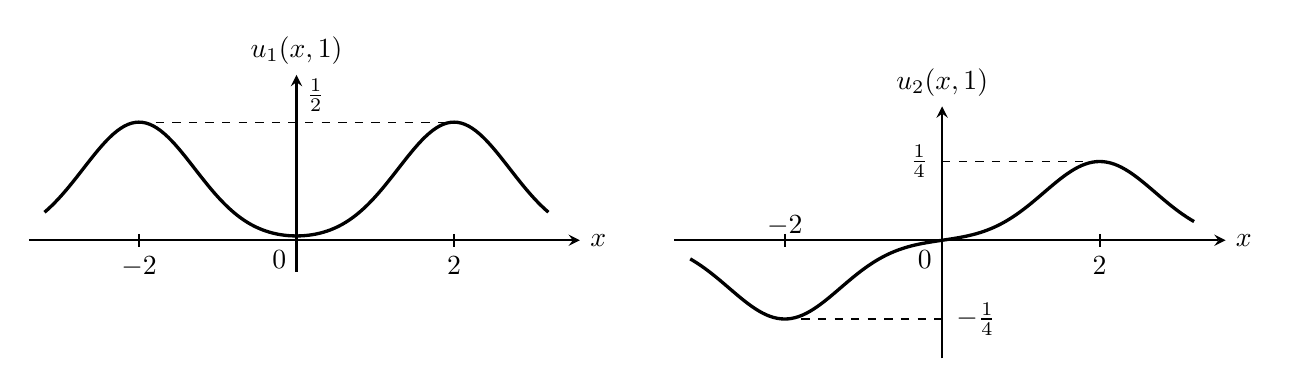
\begin{tikzpicture}[>=stealth, thick, scale=1.0]
  % Left: u_1(x, 1) = 0.5*(exp(-(x-2)^2) + exp(-(x+2)^2))
  \begin{scope}[xshift=0cm]
    \draw[->] (-3.4, 0) -- (3.6, 0) node[right] {$x$};
    \draw[->] (0, -0.4) -- (0, 2.1) node[above] {$u_1(x, 1)$};
    \node[below left] at (0, 0) {$0$};

    % Peak height 1/2 -> y = 1.5
    \draw[dashed, thin] (-2.0, 1.5) -- (2.0, 1.5);
    \node[above right] at (0, 1.5) {$\tfrac{1}{2}$};

    % Ticks at -2 and 2
    \draw (-2.0, 0.08) -- (-2.0, -0.08) node[below] {$-2$};
    \draw (2.0, 0.08) -- (2.0, -0.08) node[below] {$2$};

    \draw[very thick, domain=-3.2:3.2, samples=140]
      plot (\x, {1.5 * (exp(-(\x - 2)*(\x - 2)) + exp(-(\x + 2)*(\x + 2)))});
  \end{scope}

  % Right: u_2(x, 1) = 0.25*(exp(-(x-2)^2) - exp(-(x+2)^2))
  \begin{scope}[xshift=8.2cm]
    \draw[->] (-3.4, 0) -- (3.6, 0) node[right] {$x$};
    \draw[->] (0, -1.5) -- (0, 1.7) node[above] {$u_2(x, 1)$};
    \node[below left] at (0, 0) {$0$};

    % Peak height +/- 1/4 -> y = +/- 1.0
    \draw[dashed, thin] (0, 1.0) -- (2.0, 1.0);
    \node[left] at (-0.05, 1.0) {$\tfrac{1}{4}$};
    \draw[dashed, thin] (-2.0, -1.0) -- (0, -1.0);
    \node[right] at (0.05, -1.0) {$-\tfrac{1}{4}$};

    % Ticks at -2 and 2
    \draw (-2.0, 0.08) -- (-2.0, -0.08) node[above] {$-2$};
    \draw (2.0, 0.08) -- (2.0, -0.08) node[below] {$2$};

    \draw[very thick, domain=-3.2:3.2, samples=140]
      plot (\x, {1.0 * (exp(-(\x - 2)*(\x - 2)) - exp(-(\x + 2)*(\x + 2)))});
  \end{scope}
\end{tikzpicture}
\end{document}
